\documentclass{book}

\usepackage[utf8]{inputenc}
\usepackage[T1]{fontenc}
\usepackage{lmodern}
\usepackage[UKenglish]{babel}
\usepackage{graphicx}
\usepackage{ifthen}
\usepackage{alltt}
\usepackage{xspace}
\usepackage{amssymb}
\usepackage{amsfonts}
\usepackage{amsmath}
\usepackage{fancyhdr}
\usepackage{hyperref}
\usepackage[]{glossaries}
\usepackage{pdfpages}
\usepackage{fixltx2e} % for \textsuperscript
\usepackage{color}
\newboolean{showcomments}
\setboolean{showcomments}{true}
\ifthenelse{\boolean{showcomments}}
  {\newcommand{\bnote}[2]{
	\fbox{\bfseries\sffamily\scriptsize#1}
    {\sf\small$\blacktriangleright$\textit{#2}$\blacktriangleleft$}
    % \marginpar{\fbox{\bfseries\sffamily#1}}
   }
   \newcommand{\cvsversion}{\emph{\scriptsize$-$Id: macros.tex,v 1.1.1.1 2007/02/28 13:43:36 bergel Exp $-$}}
  }
  {\newcommand{\bnote}[2]{}
   \newcommand{\cvsversion}{}
  } 


\newcommand{\here}{\bnote{***}{CONTINUE HERE}}
\newcommand{\nb}[1]{\bnote{NB}{#1}}
\newcommand{\fix}[1]{\bnote{FIX}{#1}}
%%%% add your own macros 

\newcommand{\ab}[1]{\bnote{Alex}{#1}}
\newcommand{\sd}[1]{\bnote{Stef}{#1}}
\newcommand{\ja}[1]{\bnote{Jannik}{#1}}
\newcommand{\md}[1]{\bnote{MD}{#1}}
\newcommand{\jr}[1]{\bnote{JRe}{#1}}
\newcommand{\ben}[1]{\bnote{Ben}{#1}}

\graphicspath{{figures/}}
%%% 


\newcommand{\figref}[1]{Figure~\ref{fig:#1}}
\newcommand{\figlabel}[1]{\label{fig:#1}}
\newcommand{\tabref}[1]{Table~\ref{tab:#1}}
\newcommand{\layout}[1]{#1}
\newcommand{\commented}[1]{}
\newcommand{\secref}[1]{Section \ref{sec:#1}}
\newcommand{\seclabel}[1]{\label{sec:#1}}

%\newcommand{\ct}[1]{\textsf{#1}}
\newcommand{\stCode}[1]{\textsf{#1}}
\newcommand{\stMethod}[1]{\textsf{#1}}
\newcommand{\sep}{\texttt{>>}\xspace}
\newcommand{\stAssoc}{\texttt{->}\xspace}

\newcommand{\stBar}{$\mid$}
\newcommand{\stSelector}{$\gg$}
\newcommand{\ret}{\^{}}
\newcommand{\msup}{$>$}
%\newcommand{\ret}{$\uparrow$\xspace}

\newcommand{\myparagraph}[1]{\noindent\textbf{#1.}}
\newcommand{\eg}{\emph{e.g.,}\xspace}
\newcommand{\ie}{\emph{i.e.,}\xspace}
\newcommand{\ct}[1]{{\textsf{#1}}\xspace}


\newenvironment{code}
    {\begin{alltt}\sffamily}
    {\end{alltt}\normalsize}

\newcommand{\defaultScale}{0.55}
\newcommand{\pic}[3]{
   \begin{figure}[h]
   \begin{center}
   \includegraphics[scale=\defaultScale]{#1}
   \caption{#2}
   \label{#3}
   \end{center}
   \end{figure}
}

\newcommand{\twocolumnpic}[3]{
   \begin{figure*}[!ht]
   \begin{center}
   \includegraphics[scale=\defaultScale]{#1}
   \caption{#2}
   \label{#3}
   \end{center}
   \end{figure*}}

\newcommand{\infe}{$<$}
\newcommand{\supe}{$\rightarrow$\xspace}
\newcommand{\di}{$\gg$\xspace}
\newcommand{\adhoc}{\textit{ad-hoc}\xspace}

\usepackage{url}            
\makeatletter
\def\url@leostyle{%
  \@ifundefined{selectfont}{\def\UrlFont{\sf}}{\def\UrlFont{\small\sffamily}}}
\makeatother
% Now actually use the newly defined style.
\urlstyle{leo}





%UGLY
%%NA: Regarde la commande \hspace{some-width} et aussi \mbox[some-width]{}
\newcommand{\tab}{\mbox{ }\mbox{ }\mbox{ }\mbox{ }\mbox{ }\mbox{ }\mbox{ }}


%\hypersetup{}	% pour ne pas afficher les cadres rouges
		        	% attention, les liens seront invisibles !

\hypersetup{
    colorlinks=false,
    pdfborder={0 0 0},
}

\makeglossaries
\glossarystyle{long3col}

\newglossaryentry{Smalltalk}{name={Smalltalk},description={\emph{Smalltalk} is an object-oriented, reflective, dynamically typed, \textit{all is object} programming languages.}}

\newglossaryentry{primitive}{name={primitive},description={A \emph{primitive} is a C implemented method directly interpreted by the VM.}}

\newglossaryentry{Pharo}{name={Pharo},description={\emph{Pharo} is a fork of Squeak, an implementation of the object-oriented, dynamically typed, reflective programming language Smalltalk.}}

\newglossaryentry{Special Objects Array}{name={Special Objects Array},description={The \emph{Special Objects Array} is an array shared by the image and the VM which store primordial information.}}

\newglossaryentry{Garbage Collector}{name={Garbage Collector},description={The \emph{Garbage Collector} is a mechanism which consist in automatically destroy unreferenced objects of a living system in order to recover memory.}}

\newglossaryentry{Micro Squeak}{name={Micro Squeak},description={\emph{Micro Squeak} is a \emph{John Maloney}'s project which produces a headless 57k image with a few basic classes as a proof of concept.}}

\newglossaryentry{Moose}{name={Moose},description={\emph{Moose}  is a platform for software and data analysis maintained by a part of the RMoD team.}}

\newglossaryentry{SVN}{name={SVN},description={\emph{Subversion} is a tool for version control.}}


                 
% ------------------------------------------------------------------------ 	%
%											%
%				     Acronyms					%
%											%
% ------------------------------------------------------------------------ 	%

\newacronym[\glsshortpluralkey=VM,\glslongpluralkey=Virtual Machine]{VM}{VM}{Virtual Machine}

\newacronym[\glsshortpluralkey= IDE,\glslongpluralkey= IDE]{IDE}{IDE}{Integrated Development Environment}

\newacronym[\glsshortpluralkey= SOA,\glslongpluralkey= SOA]{SOA}{SOA}{Special Objects Array}

\newacronym[\glsshortpluralkey= IUT,\glslongpluralkey= IUT]{IUT}{IUT}{Institut Universitaire de Technologie}




\begin{document}
\makeatletter
               
\renewcommand{\cleardoublepage}{%
		\clearpage\ifodd\c@page\else
		\hbox{}
		\vspace*{\fill}
		\thispagestyle{empty}
		\newpage
		\fi}

 \renewcommand\tableofcontents{%
     \if@twocolumn
       \@restonecoltrue\onecolumn
     \else
       \@restonecolfalse
     \fi
     \section*{\contentsname
         \@mkboth{%
            \MakeUppercase\contentsname}{\MakeUppercase\contentsname}}%
     \@starttoc{toc}%
   	\thispagestyle{empty}
     \if@restonecol\twocolumn\fi
     }


\fancypagestyle{plain}{%
	\fancyhf{}
	\renewcommand{\headrulewidth}{0pt}
	\renewcommand{\footrulewidth}{0pt}
	}

\newcommand\resume{\@startsection {subsection}{1}{\z@}%
                                   {-3.5ex \@plus -1ex \@minus -.2ex}%
                                   {2.3ex \@plus.2ex}%
                                   {\normalfont\Large\bfseries\hfil}}

%\renewcommand\l@section[2]{%
%  \ifnum \c@tocdepth >\z@
%    \addpenalty\@secpenalty
%    \addvspace{1.0em \@plus\p@}%
%    \setlength\@tempdima{1.5em}%
%    \begingroup
%      \parindent \z@ \rightskip \@pnumwidth
%      \parfillskip -\@pnumwidth
%      \leavevmode {\bfseries
%      \advance\leftskip\@tempdima
%      \hskip -\leftskip
%      #1}\nobreak\ 
%      \leaders\hbox{$\m@th\mkern \@dotsep mu\hbox{.}\mkern \@dotsep mu$}
%     \hfil \nobreak\hb@xt@\@pnumwidth{\hss #2}\par
%    \endgroup
%  \fi}
  	
\newcommand\warning[1]{\par\textcolor{red} {\large \MakeUppercase{#1} \normalsize}}
\newcommand\goal{\paragraph{Goal:}}
\newcommand\problems{ \paragraph{Problems:}}
\newcommand\solutions{\paragraph{Solutions:}}
\newcommand\inanutshell{\paragraph{In a nutshell:}}


\makeatother

\title{Hazelnut: bootstrapping a reflective kernel}
\author{Benjamin Van Ryseghem}

%\maketitle

\includepdf{figures/Cover.pdf}
\section*{Thanks}
\begin{itemize}
	\item[] \hspace{-0.5cm}I would like to especially thank St\'{e}phane Ducasse and Jannik Laval who have always been there to show me the way, and answer my questions.
	\item[] \hspace{-0.5cm}I also would like to thank Jean-Baptiste Arnaud and Igor Stasenko who have spent hours explaining to me how the VM works.
	\item[] \hspace{-0.5cm}I would like to thank the whole team. It was a real pleasure to work with you.
	\item[] \hspace{-0.5cm}I also would like to thank the reviewers: Damien Pollet, \ben{to fill}
\end{itemize}
\newpage



\addcontentsline{toc}{section}{Abstract}
\vfill 

\resume*{R\'{e}sum\'{e}}

Dans le cadre de mon stage de fin d'\'{e}tudes, j'ai eu en charge le projet \textbf{Hazelnut} au sein de l'\'{e}quipe RMoD au sein de l'INRIA (Institut National de Recherche en Informatique et en Automatique) de Lille. Le projet Hazelnut consiste en la cr\'{e}ation dynamique d'un nouveau noyau d'ex\'{e}cution \`{a} partir d'une \mbox{impl\'{e}mentation} de Smalltalk, Pharo. 

Ce projet doit permettre de concevoir aisement des noyaux minimaux pouvant servir \`{a} des syst\`{e}mes embarqu\'{e}s aussi bien qu'\`{a} red\'{e}finir facilement la fa\c{c}on dont le noyau (et donc le syst\`{e}me) fonctionne.


\vfill

\resume*{Abstract}

During my internship at INRIA (Institut National de Recherche en Informatique et en Automatique) in the RMoD team, I had in charge the \textbf{Hazelnut} project which consists in the dynamic creation of a new kernel from Pharo, an implementation of Smalltalk.

This project will be used to create minimal kernel for embedded systems or to easily redefine the way the kernel (and the whole system) works.

\vfill

\newpage


\newpage


%%NA GROS rpoblemes d´ indentation dans la table des matieres.
%% A tros redefinir de trucs on finit par tout casser le pauvre style LaTeX
%% Il semble aussi y avoir des probleme d'espaces apres tes numero de section
\tableofcontents
%\mainmatter

\newpage


%------------------------------------------------------------%
%									%
%			INTRODUCTION			%
%									%
%------------------------------------------------------------%

\chapter{Introduction}Currently student at the \emph{Universit\'{e} Lille 1} at Villeneuve d'Ascq in the sixth semester of the licence Informatique\footnote{a computer science formation in three years} I had to do an internship for graduation in a research laboratory from 1st April 2012 to 31th June 2012. I have done this internship in the RMoD team working for the Inria, formerly named INRIA for "Institut National de Recherche en Informatique et en Automatique". I already did my DUT graduation internship \footnote{from 1st Novembre 2010 to 1st April 2011} is this team on the same project.

Few weeks before the beginning of my previous intership, \emph{John Maloney} released one of his projects named \gls{Micro Squeak} consisting in a proof of concept of the creation of a new kernel (the core classes and methods of the system).
%%NA: ca me semble avance de parle d'image a ce moment
% and a new image based on this kernel.
We have decided to port this project in \gls{Pharo}. It is named the project \emph{Seed}.

\paragraph{Context:}
%%NA: added some sentences to clarify things here and later
Smalltalk is an object-oriented language that has the property to save the entire state of the environment from one session to the other in a file called an image. An image contains a snapshot of the Smalltalk environment's memory. It basically contains all the classes and objects of the system at the moment it was saved. The Smalltalk environment is a ``living thing'', it is never created from scratch, but every new version is evolved from a previous image. For example, there are very probably in all current smalltalk images, objects that were created back in the first version of the first Smalltalk in the 70's (e.g. the ``true'' and ``false'' objects).
%%NA: end of additions
%NA: ne pas mettre le nom en italic.
After \emph{John Maloney}'s project was released, we had a proof that the creation of a new kernel was possible, and we wanted to have this concept in \gls{Pharo}. Some other projects\footnote{mainly Chacharas, Spoon } have provided the tools to create new kernels, but with a different approach. \emph{Seed} is the first project inspired by \gls{Micro Squeak}.

\paragraph{Problems:}
The problems are that \gls{Micro Squeak} is based on the version 3.7 of Squeak, and even if the project has been released few months ago, it had been developed in 2004. Due to that the project is not synchronized with the lastest evolutions of the system anymore. Moreover, the system I used during my internship \gls{Pharo}, is a fork of Squeak. Pharo already got a large refactoring effort but it is still a monolithic system, with still a lot of useless or inefficient code. Because of that, it's quite difficult to define properly what the kernel is and to extract it without collecting irrelevant classes.

\paragraph{Goals}
The goal of the Hazelnut project is to automatically extract a kernel from a living \gls{Pharo} image and to bootstrap this kernel into an image. The process has to be automatic to be able to follow the \gls{Pharo} evolution. Moreover, in order to ease the kernel creation process, the \gls{Pharo} structure has to be fixed. So in a nutshell the goals of the project are:
%%NA: Fort all lists: ";"at the end of each item, "."at the end of the last item, capital at the beginning of each item
	\begin{itemize}
		\item Identify a kernel for \gls{Pharo};
		\item Automatize this identification;
		\item Fix the \gls{Pharo} structure;
		\item Make the two last tasks in parallel because the system (and therefore its kernel) is currently evolving and under heavy modifications;
		\item Bootstrap a new image with this kernel.
	\end{itemize}
Such a kernel could be used in embedded devices, due to the lightweight of the new image, or be used to modify the kernel of the system and to restart from this new kernel without old living objects. It's an argument for the agility of \gls{Pharo}.

\paragraph{Contributions:}
My contributions to this project was to:
	\begin{itemize}
		\item Initiate the project;
		\item Write a kernel extraction script;
		\item Write kernel analysis tools;
		\item Work on \gls{Pharo} kernel analysis to define the kernel;
		\item Work on the whole \gls{Pharo} system to flag the system weaknesses such as wrong dependencies between packages;
		\item Work on different ways to generate a new image;
		\item Write unit tests;
		\item Reduce the generated image size;
		\item Set the initialization
		\item Ensure the reinitialization of the generated system;
		\item Fix the system, especially the \gls{Pharo} kernel.
	\end{itemize}
During my internship, I also worked on the integration of some tools of mine and on their maintenance.

	
%------------------------------------------------------------%
%									%
%			       CONTEXT    			%
%									%
%------------------------------------------------------------%

\chapter{Context}

Firstly I will introduce the work environment I used to live in during my internship in three parts, the institution I was working for, the team I was working in and the language I was working with.

	\section{Inria}\paragraph{Presentation:} Inria is a french institution under the dual supervision of the ministries of research and industry which goal is to undertake research in basic and applied sciences and information technologies and communication (SITC). The institute also provides a strong technology transfer in a close attention to training through research, dissemination of scientific and technical development, expertise and participation in international programs.

\paragraph{Composition: } Inria accommodates 3800 people in its eight research centers located in Rocquencourt, Rennes, Sophia Antipolis, Grenoble, Nancy, Bordeaux, Lille and Saclay, 2800 of them are scientists from Inria and partner organizations (CNRS, universities, colleges) working in over 160 project teams of joint research. Many Inria researchers are also professors and their students (about 1000) are preparing their thesis within the project teams of Inria research.

\paragraph{The research center of Lille: } The Inria Lille -- Nord Europe, led by David Simplot-Ryl, gathers from its creation 10 research teams located in a building of 4000m$^2$ acquired with the help of local government and European funds. It hosts more than 220 people, nearly half is paid by the Institute. This Inria  center is an asset for the competitiveness of Nord - Pas de Calais in research and innovation.

	\section{The RMoD Team}\paragraph{Presentation: } The goal of the RMoD team is to help re-modularization of object-oriented applications. This goal follows two complementary lines: re-engineering and definition of new constructors for programming languages. To help re-engineering, new analyses are proposed in order to understand and remodularize big applications (specialized metrics, adapted visualizations, \emph{etc}). In the context of programming languages, constructors for the modularity features and new systems modules validation are performed. The team is also working on a secured kernel for Pharo, an \gls{IDE} for Smalltalk used and maintained by the team.
%%NA: Ca donne l'impression que pharo est exclusivement un projet de l'equipe.
%%quelque chose comme "used by the team which is also an active member of its community"

\paragraph{Applications re-modularization: } The evolution of an application is limited by strong dependencies between its inner parts. That's why it's crucial to answer the following questions:
%%NA: ne pas utiliser " mais `` et ''
\emph{``How can we substitute a part by another one with minimal impact~?''}, \emph{``How to identify reusable elements~?''} or \emph{``How to modularize an application when there is wrong links~?''}. To answer those questions is the goal of Moose, the team software analysis environment, provides a set of analyses.
%%NA: de nouveau ce n'est pas l'environnement de l'equipe, c'est un environnement que nous utiliser et dont nous faisont parti de la comunauté ...
This work is divided in tree parts :
	\begin{itemize}
		\item Tools to understand big applications (packages/modules);
		\item Analysis for remodularization;
		\item Software quality.
	\end{itemize}
	
\paragraph{Semantics elements for modularity.} This second line focuses on the definition of new semantics elements for languages in order to construct flexible and reconfigurable software. The team continues its efforts on Traits and Classboxes but also works on new areas such as security in dynamic languages. It works on:
	\begin{itemize}
		\item The definition of a \emph{Traits-only} language and;
		\item Reconciliation between reflexive languages and security.
	\end{itemize}
	\section{Smalltalk presentation in a nutshell}\emph{\gls{Smalltalk}} is the language used in the team, therefore this is the language I used during my internship. To understand the challenges I faced I will briefly present \gls{Smalltalk} and its main characteristics.

\subsection {What is Smalltalk ?}

\emph{\gls{Smalltalk}} is an object-oriented, reflective, dynamically typed programming languages. So let's explain each word:

%@@NO SPACE before :?; in english@@

\begin{itemize}
	\item Object-oriented : in \gls{Smalltalk}, you manipulate objects which send messages (like in Java or C++);
	\item Reflective : each object can inspect or modify its own structure at runtime (like Java, but to a much greater extent);
	\item Dynamically typed : variables don't have a type at compilation, but only when a value is stored in them at runtime;
	\item \textit{Everything is an object}: everything is an object (a class, a message, a method, \dots)
\end{itemize}

\subsection{Smalltalk basics}

\gls{Smalltalk} is based on 2 classes which constitute the conceptual core of this system, \ct{Object} and \ct{Class} (see Figure~\ref{ClassObjectBootStrap}). Here you can see that each element cannot exist alone. The bootstrap is the process which leads to this state. However, since \ct{Class} and \ct{Object} needs other objects such as string, characters, stream, numbers\dots the real bootstrap is more complex.

\begin{figure}[h]
	\centering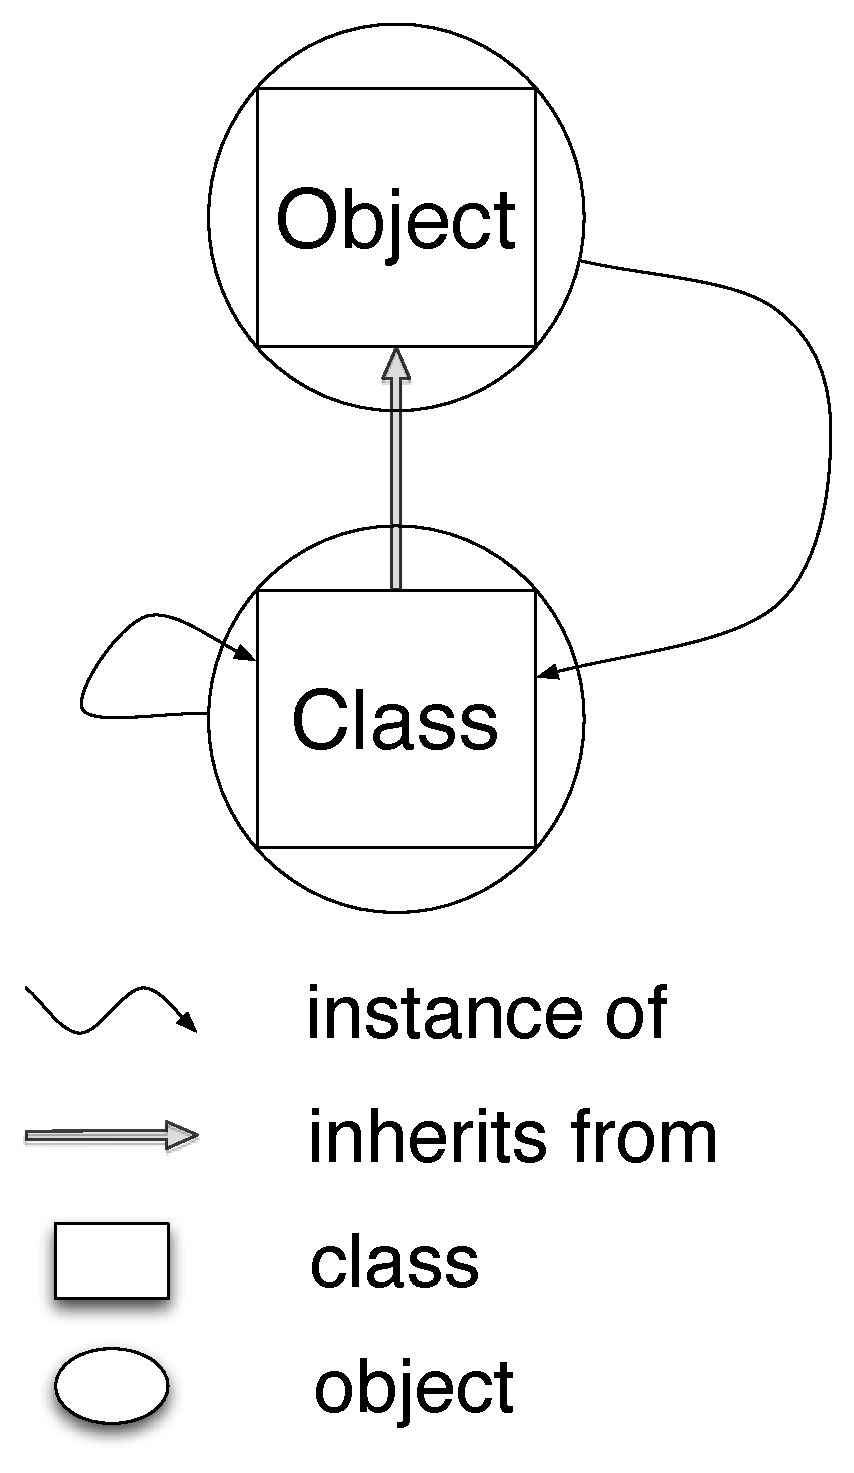
\includegraphics[height = 7cm]{figures/BootStrap}
	\caption{Class and Object bootstrap}
	\label{ClassObjectBootStrap}
\end{figure}
	
The most important thing to know is that a bootstrap is a process where a system is initializing itself via its own execution. It's close to the \emph{Chicken or egg dilemma} where each one deeply depends on the other one (more details will be given in the next chapter, page~\pageref{BootStrap}).

\subsection{Some basics code lines}

Here few examples of \gls{Smalltalk} code to know how to read further examples:

\begin{code}{}
	"Variables declaration"
	| variable1 variable2 |

	"Instance creation"
	variable1 := Point new.
	"Instance setting"
	variable1 x: 1.
	variable1 y: 2.
	
	variable2 := Point new.
	variable2 x: 1.
	variable2 y: 2.
	
	variable1 = variable2. \emph{true}
	variable1 == variable2. \emph{false}
\end{code}
Here, we can see 5 things :
\begin{itemize}
	\item \ct{| |} : it allows you to declare variables.
	\item \ct{:=} : it is the assignment.
	\item \ct{new} : it's a class method which creates a new instance of the receiver, e.g. ``\texttt{Point new}'' sends the message new to the class (which is also an object) Point.
	\item \ct{=} : it tests if two objects represent the same object, it's a \emph{logical} equality. It is a message, asking the receiver (before =) whether it is the same object as the parameter (after the =).
	\item \ct{==} : it tests if two objects point to the same reference, it's a \emph{physical} equality. It is a message also.
\end{itemize}
Let's see a basic method of the \ct{Integer} class:

\begin{code}{}
plus: integer1 andPlus: integer2 

\tab^ self + integer1 + integer2
\end{code}
Here we learn 3 new things:
\begin{itemize}
	\item \ct{:} : the way to specify parameters to most methods.
	\item \ct{self} : the receiver of the method (similar to this in Java).
	\item \ct{\^} : it allows you to return a value\footnotemark. By default a method returns \ct{self}.
\end{itemize}
\footnotetext{You can sometime see $\uparrow$ instead.}
A method is often referred to by the notation \ct{Class$\gg$\#selector} to have an unique notation. So the method we just saw is noted \ct{Integer$\gg$\#plus:andPlus:}. 
One more example to see the last syntax elements, a method of class \ct{Class}:
\begin{code}{}
copyMethodDictionary
	   "This method answer a copy of my method dictionary"
	
	   | result |
	   result := SortedCollection new sort: [:m1 :m2 | m1 selector < m2 selector].
	   self methodDictionary do: [:method |
	       result add: method.
	       Transcript  show: method selector asString, ' added.';cr].
       ^ result
\end{code}
Here we have :
\begin{itemize}
	\item \ct{"some text"} : a comment.
	\item \ct{[:arg | code]} : it's a block (a $\lambda$-expression). They act like anonymous methods where arg is an argument of the block which is used to execute the code. In addition it captures its creation environment - it is a lexical closure.
	\item \ct{rcvr m1; m2} : it's a cascade of messages. It means that the receiver of the second method (m2) is the same that the first method's (m1) receiver, in this case \ct{rcvr}.
\end{itemize}

Now, you know the syntax of \gls{Smalltalk}.

\subsection{The SystemDictionary}

The \emph{System Dictionary} is a dictionary which contains all the global variables, including all the classes of the system. In \gls{Pharo}, the variable \emph{Smalltalk} is, normally, the sole SystemDictionary of the system. We can notice that \emph{Smalltalk} is a global variable, so it contains itself.

\subsection{Special Object Array}

The \gls{Special Objects Array} is basically an array shared between an image and the \gls{VM}. It's an interface allowing the \gls{VM} to know where are special objects it needs.

\paragraph{What is in the Special Objects Array ?}
Here I will give the first ten elements of the \gls{Special Objects Array}:
\begin{itemize}
	\item \ct{nil}\footnote{\ct{nil} is te basic NullPattern object, like \ct{NULL} in C or \ct{null} in Java} 
	\item \ct{true}
	\item \ct{false}
	\item \ct{\#Processor->Processor}
	\item \ct{Bitmap}
	\item \ct{SmallInteger}
	\item \ct{ByteString}
	\item \ct{Array}
	\item \ct{Smalltalk}
	\item \ct{Float}
	\item \dots
\end{itemize}

We can notice that the nineth element is \ct{Smalltalk}, the current SystemDictionary.

\subsection{The Virtual Machine}

As some other languages (especially Java), Smalltalk's methods are converted then interpreted by a \gls{VM}. In fact, the Smalltalk compiler analyzes the code then createss a \ct{CompiledMethod} which is a representation of the method but including more information ready to be executed by a \emph{byteCode} interpreter or JustInTime translator:
\begin{itemize}\label{literal}
	\item the \emph{byteCode} : the source code converted into a language that the \gls{VM} can interpret;
	\item the \emph{literals} : they represent low level objects such as number true, false, strings that are referenced and read by the scanner at compilation time. \emph{Literals} especially store pointers to class referred into the source code.
\end{itemize}

\subsubsection*{Method}
Let's see an example, \ct{String$\gg$\#copy} :

\begin{code}{}
copy

\tab | string |
\tab string := String new: (self size).
\tab self doWithIndex: [:character :index |
\tab \tab string at: index put: character].
\tab ^ string
\end{code}

First, let's explain what this method do :

\begin{itemize}
	\item \ct{| string |} : we declare a new variable named \ct{string}.
	\item \ct{string := String new: (self size)} : it creates a new instance of the class \ct{String} which the size is set at the size of the receiver and then stores it in the variable named \ct{string}.
	\item \ct{self doWithIndex: [:character :index |} : we browse the receiver and for each element, we store the element in the variable \ct{character} end the index of the element in the variable \ct{index}.
	\item \ct{string at: index put: character} : at the index \ct{index} of \ct{string}, we put \ct{character}.
	\item \ct{\^{} string} : we finally return the variable \ct{string}.
\end{itemize}
In a nutshell, this method basically parses the receiver (which is a \ct{String}) and fills up a new \ct{String} with the same value.

\subsubsection*{CompiledMethod}
Now, let's take a look at the corresponding \ct{CompiledMethod}
\begin{itemize}
	\item the \emph{byteCode} : 
	\begin{code}{}
		21 <40> pushLit: String
		22 <70> self
		23 <C2> send: size
		24 <CD> send: new:
		25 <68> popIntoTemp: 0
		26 <70> self
		27 <10> pushTemp: 0
		28 <8F 12 00 05> closureNumCopied: 1 numArgs: 2 bytes 32 to 36
		32 	<12> pushTemp: 2
		33 	<11> pushTemp: 1
		34 	<10> pushTemp: 0
		35 	<C1> send: at:put:
		36 	<7D> blockReturn
		37 <E1> send: doWithIndex:
		38 <87> pop
		39 <10> pushTemp: 0
		40 <7C> returnTop
	\end{code}
	Basically, the \emph{byteCode} tells the \gls{VM} how to manage the execution stack. 
		\item the \emph{literals} : 
		\begin{itemize}
			\item \ct{\#String->String} : this literal refers to the String called at the instantiation of \ct{String}. This association is the one present in the \gls{Pharo} SystemDictionary
			\item \ct{\#doWithIndex:} : this literal refers to a method invoked.
			\item \ct{\#copy} : this literal represent the selector of the method. It doesn't appear in the \emph{byteCode} because it's not needed (moreover, historically, methods used to be anonymous).
			\item \ct{\#String->String} : this literal refers to the class of the method.
		\end{itemize}
		You can notice that \ct{new} and \ct{at:put:} are not in the literal. It is due to the fact that those methods are \emph{special byteCodes}
\end{itemize}

It's important to keep in mind that all methods points to the current SystemDictionary through their literals, but you do not have to be able to read or understand the \emph{byteCode} because it's a very low level tool. Moreover, \emph{byteCode} is rarely read by developers.


%------------------------------------------------------------%
%									%
%			BOOTSTRAPPING			%
%									%
%------------------------------------------------------------%

\chapter{Bootstrapping Challenges}

In this chapter we first define what is a system bootstrap and give some related definitions, then we present the current problems and the goals of our work.

	\section{Definitions and benefits}\paragraph{Reflective system.}

%De nombreux langages r\'eflexifs sont apparus ces derni�res ann\'ees : langages
%objets \cite{Maes87a, Bobr86a, Coint87a, Coint89a, Chiba93a, Danforth94a,
%Chiba95, Brandt96, Rivard96b}, langages d'acteurs \cite{Ferber84,Ferber88,
%Ferber93, Briot94, Briot96}, programmation concurrente \cite{Yonezawa88,
%Ishikawa91,Yonezawa92, Yonezawa92b}, langages � prototypes \cite{Mulet93a,
%Mulet93b, Mulet95}.  L'utilisa\-tion de protocoles m\'eta-objet a permis de mettre
%en place des m\'ecanismes vari\'es comme des types de donn\'ees atomiques
%\cite{Stroud95}, l'introduction d'objets persistants \cite{Paepcke90}, des
%bo�tes � outils graphiques \cite{Rao91,Gallesio96} et la construction de
%syst�mes d'exploitation.  Apr�s avoir pos\'e le vocabulaire, nous analysons les
%besoins qui ont favoris\'e l'\'emergence des syst�mes dit {\em ouverts}.  Nous
%abordons ensuite les difficult\'es sp\'ecifiques � la conception de ces syst�mes.
%Nous pr\'esentons rapidement deux protocoles m\'eta-objet (MOP) en pr\'esentant
%celui de \Clos \cite{Kiczales91} et de \CodA \cite{McJaffer95}.  Nous avons
%choisi \Clos car son MOP constitue la r\'ef\'erence en la mati�re, mais aussi le
%MOP nomm\'e \CodA qui choisit une factorisation des m\'eta-comportements originale
%et plus g\'en\'erale centr\'ee autour du concept d'objet. 
%

%\section{Concepts et d\'efinitions}
%\mcite{La r\'eflexion d\'esigne l'ensemble des pr\'eoccupations visant � rendre
%visible dans le langage certains m\'ecanismes internes.}{Mulet95}
%
%La r\'eflexion est � la base des langages ouverts.  Ce concept qui ne se limite
%pas exclusivement aux langages � objets existe aussi en programmation logique
%ou fonctionnelle \cite{Demers95}.  \Smith fut le premier � introduire un tel
%concept dans un langage de programmation : \tLisp, son langage r\'eflexif, \'etait
%un langage fonctionnel \Lisp \cite{Smith84}. 


Smith defines reflexivity as: {\em <<~An entity's integral ability to represent, operate on, and
otherwise deal with itself in the same way that it represents, operates on and
deals with its primary subject matter~>>}.~\cite{Bobr93a}

In the context of programming languages, this definition can be stated
as: \emph{Reflection is the ability of a program to manipulate as data
something representing the state of the program during its own
execution. There are two aspects of such manipulation : {\em introspection}
and {\em intercession} [...] Both aspects require a mechanism for encoding
execution state as data; providing such an encoding is called {\em
reification}.}~\cite{Bobr93a}


Maes has proposed in the first chapter of his thesis
\cite{Maes87b}, precise definitions to clearly characterize
reflective programming. We refer here to these definitions:

\begin{itemize}
\item A {\bf computational system} is something that {\bf reasons} about and
{\bf acts} upon some part of the world, called the {\bf domain} of the system
(p 13).

\item A computational system may also be {\bf causally connected} to its
domain. This means that the system and its domain are linked in such a way
that if one of the two changes, this leads to an effect upon the other (p 15).

\item A {\bf meta-system} is a computational system that has as its domain
another computational system, called its {\bf object-system}. [...] A
meta-system has a representation of its object-system in its data. Its
program specifies {\bf meta-computation} about the object-system and is
therefore called a {\bf meta-program} (p 17).

\item {\bf Reflection} is the process of reasoning about and/or acting upon
oneself (p 19) (see Figure~\ref{AllSystems}).

\begin{figure}[h]
	\centering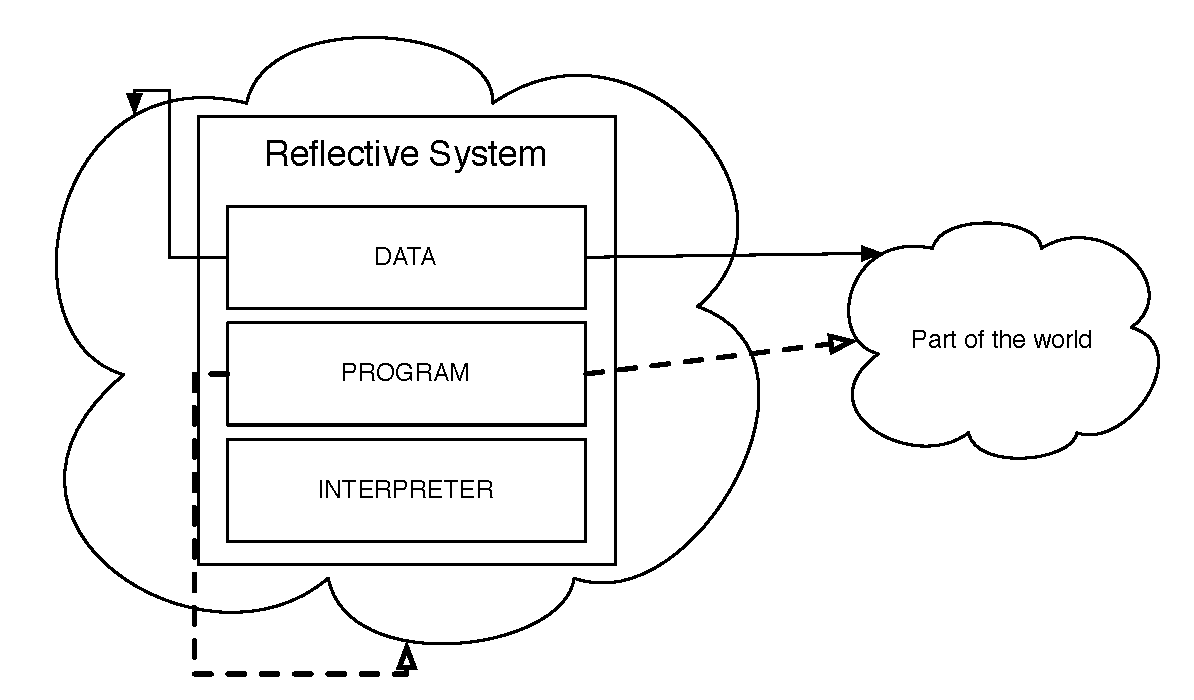
\includegraphics[width = 10cm]{figures/ReflexiveSystem}
	\caption{A Reflexive System}
	\label{AllSystems}
\end{figure}



\item A {\bf reflective system} is a causally connected meta-system that has
as object-system itself. The data of a reflective system contain, besides the
representation of some part of the external world, also a causally connected
representation of itself, called {\bf self-representation} of the
system. [...] When a system is reasoning or acting upon itself, we speak of
{\bf reflective computation} (p 19).

\item A language with a {\bf reflective architecture} is a language in which
all systems have access to a causally connected representation of themselves.

\item A programming environment has a {\bf meta-level architecture} if it has
an architecture which supports meta-computation, without supporting reflective
computation (p 34).
\item The {\bf meta-object} of an object X represents the explicit information
about X (e.g. about its behavior and its implementation). The object X itself
groups the information about the entity of domain it represents (p 120).
\end{itemize}

\paragraph{Bootstrap.}
Bootstrapping a kernel is the process that builds the minimal structure of a language that is reusable to define this language.
The idea is to use as early as possible the benefits of the resulting language by implementing a minimal core whose only goal is to be able to build the full system. As an example of a possible bootstrap: we write in C the minimal structures to represent and execute objects, and we then write with this core the full system. This avoids to have to write the full system (compiler for example in C). In ObjvLisp \cite{Coin87a}, the class Class is first defined using low level API, then Object is created, then Class is fully reimplemented using the first one.
	\section{Current problems in Pharo}The current structure of \gls{Pharo} is a problem for creating easily a bootstrap at different levels:
\begin{itemize}
	\item \gls{Pharo} has a monolithic structure with a lot of old code (even though all our efforts are on that);
	\item There are hidden structural dependencies requiring deep analysis to be revealed. For example, Stream depends on Compiler while it should be the inverse;
	\item The definition of what is part of the \gls{Pharo} kernel is fuzzy and dispatched through different packages which aren't autonomous and self contained.
\end{itemize}\label{BootStrap}
	\section{Goals of the project}\paragraph{Bootstrapping.} We need a process to create an autonomous kernel and to bootstrap it into a new image. This process has to be modular in order to be able to create a specific kernel.
This kernel has to be autonomous which means it has to be isolated from the other classes and can only refer to itself.

\paragraph{Dealing with kernel changes.}
Pharo development is real active in all parts of the system and in particularly the kernel. Therefore it is not possible to take 6 or 8 months to just bootstrap it.
We need a solution that can cope with the continuous changes and fixes in the kernel. 


\paragraph{}Therefore we will attack the problem from two angles: (1) cleaning the current kernel to ease the bootstrap, (2) building a bootstrap process that can be applied to the evolving kernel.


%------------------------------------------------------------%
%									%
%				HAZEL				%
%									%
%------------------------------------------------------------%
\chapter{Hazelnut}

Hazelnut is one of the \textbf{Seed} projecst, where \textbf{Seed} was originally composed by different projects whose goal is to generate new kernels, all based on the project \emph{Micro-Squeak}.
For now we essentially distinguish two of them:
\begin{itemize}
	\item PineKernel: it is a port of \gls{Micro Squeak} in Pharo
	\item Hazelnut: it is the building of a kernel in Pharo starting from the Pharo kernel.
\end{itemize}

This project is composed by three different parts, the kernel collection, the kernel isolation and finally the image creation.

	\section{Kernel creation}%I have quickly decided to collect the kernel by collecting classes, copying them (without recompiling them) in a new SystemDictionary, and then to fix all the references. 
%
%The point was which classes have to be collected. For my first attempts, I just tried to collect all classes Object depends on. I knew it will be huge, but at least I will not have dependencies to object not in my Hazel world.
%Unfortunately it was almost half of the system, and it is not effective for a minimal kernel.
%
%So I changed my point of view and decided to provide a list of classes to the builder with only the classes I want. It brings new problems, the most important one was how to fix dependencies to the old world, but moreover, it didn't answer to the question which classes should I choose.
%
%To be able to choose, I've analyze dependencies between packages. At least a package is named Kernel, so I started from this package then recursively analyze dependencies. It was quite difficult because I doesn't know the whole system very well and for each dependence, I had to choose. Due to that, I've learned a lot about the system and it structure.
%
%So at this point, I was able to select the classes then to copy them into the Hazel SystemDictionary, but references still point to \gls{Pharo} classes (see Figure~\ref{ClassesCopy}).

\goal
The goal of this part is to create an alternative SystemDictionary (a SystemDictionary is a namespace holding all the classes of the system) starting from the existing one in \gls{Pharo}, and to collect classes which are needed to build the kernel. 

\problems
\begin{itemize}
	\item Which classes need to be collected ?
	\item How do we fill up the new SystemDictionary with those classes ?
\end{itemize}

\solutions
\begin{itemize}
	\item A first naive approach is to collect every class \ct{Object} depends on in order to have an autonomous system. But due to bad dependencies in the system, the kernel collected this way contains half of the \gls{Pharo} classes. This is clearly not satisfying. Therefore we have decided to have another approach. The second and final approach is to provide to the builder the list of classes the user wants in the new kernel plus some classes absolutely needed by the system\footnote{as \ct{Object}, \ct{ProtoObject} or \ct{MethodContext} for example}. The problem is that we had to determine which classes are the absolutely needed ones. In order to answer this question, a tool to analyze classes dependencies has been written and recursively used starting from the Kernel package until we had a quite autonomous kernel composed of around 200 classes\footnote{\gls{Pharo} contains around 1800 classes}. This tool also flags bad dependencies, but this part will be exposed in the next chapter (page~\pageref{KernelIsolation}). 


	\item MicroSqueak's solution to fill up the new \ct{SystemDictionary} is to recompile needed classes with a prefix and then to collect them. It's quite efficient when you have 20 classes to copy, but here we have the constraints that we do not know by advance what we will copy and then we want to be as fast as possible. 
\end{itemize}	
	
The solution we adopted is to create a new instance of \ct{SystemDictionary} and to directly copy classes into it without recompiling them. The classes are still pointing to their original namespace as shown by Figure~\ref{ClassesCopy}.
	
\begin{figure}[h]
	\centering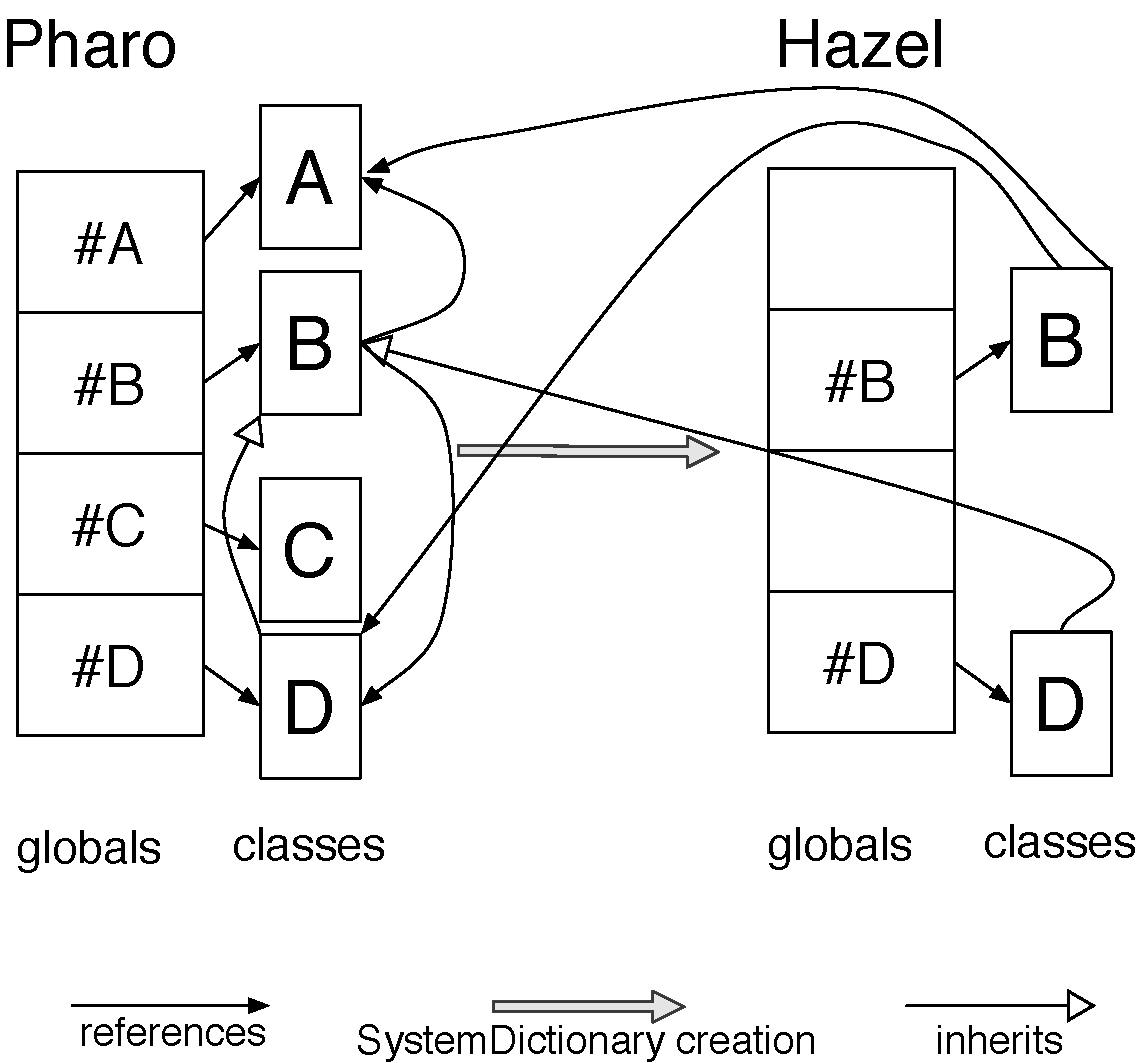
\includegraphics[width = 8cm]{figures/CopyWithInh}
	\caption{Step 1 - Copy the classes \ct{B} and \ct{D} into the new SystemDictionary}
	\label{ClassesCopy}
\end{figure}
	
The second step is to make sure that the class and metaclass hierarchy is maintained in both the environments and that the \ct{methodDictionary}\footnote{a \emph{methodDictionary} is a dictionary implemented in each class and containing all the methods of the class} is also copied. To be sure to reconstruct the hierarchy, the copy method recursively rebuild class, metaclass and superclass hierarchy (see Figure~\ref{ClassMetaClassHierarchy}).

\begin{figure}[h]
	\centering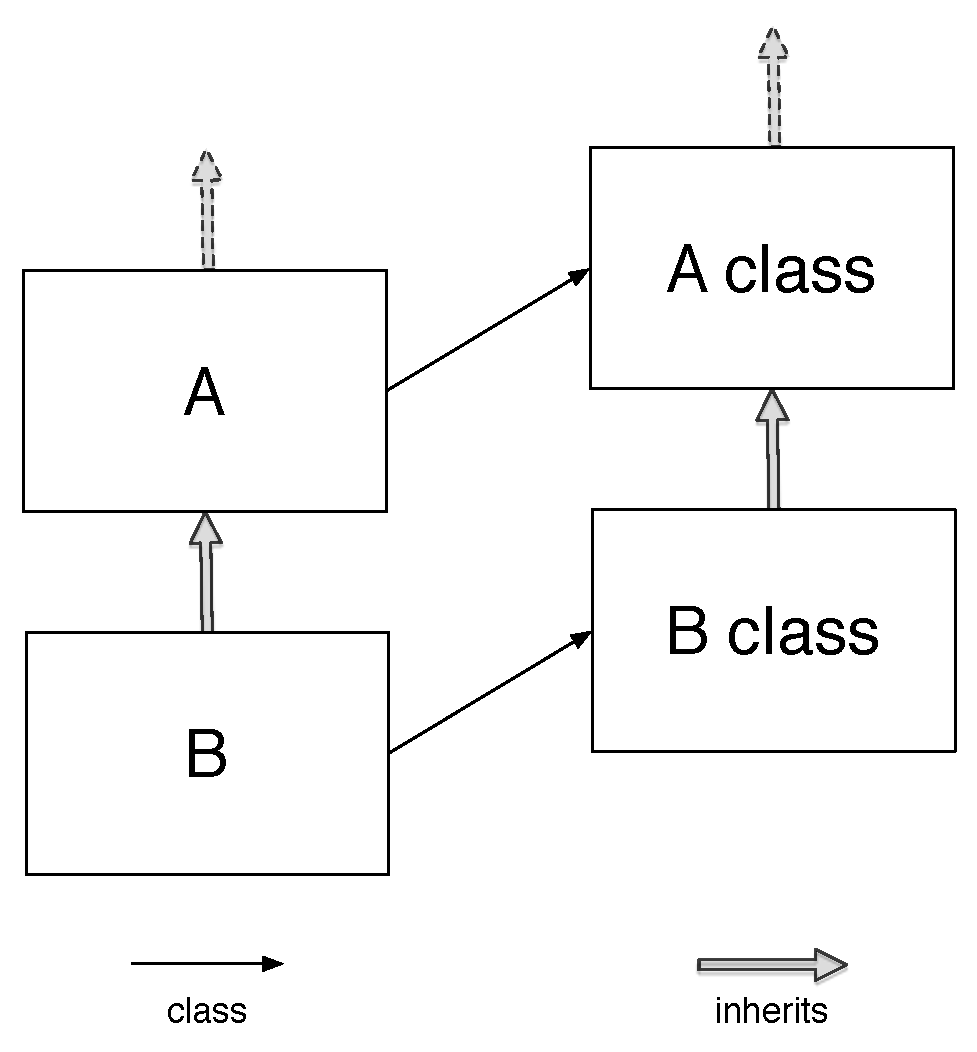
\includegraphics[width = 8cm]{figures/ClassMetaClassHierarchy}
	\caption{Class and MetaClass Hierarchy}
	\label{ClassMetaClassHierarchy}
\end{figure}

	
Here is the pseudo code in Smalltalk that add a class in the Hazel SystemDictionary and check the hierarchy:
	
	\begin{code}{}
		HazelKernelBuilder>>\#addAClassInDictionary: class
		"Add a copy of the class in the Hazel SystemDictionary then answer the copy"

		\tab| hazel copy className |
		\tab className := class name asSymbol.
	
		\tab"Check if the class is already in the dictionary"
		\tab(self list includesKey: class name) 
		\tab\tab	ifFalse: [^ nil].
	
		\tab hazel := Smalltalk at: #HazelSmalltalk.
		\tab(hazel globals includesKey: className) 
		\tab\tab	ifTrue: [^hazel at: className].

		\tab"If not, add a copy in the dictionary"
		\tab copy := self copyClass: class.
		\tab self registerClass: copy.

		\tab"then check the superclass"
		\tab copy superclass ifNotNilDo: [:superclass || superCopy | 
		\tab\tab	"add the superclass"
		\tab\tab	superCopy := self addAClassInDictionary: superclass.
		\tab\tab	"change the superclass"
		\tab\tab	copy superclass: superCopy.
		\tab\tab	"then change the metaclass's superclass"
		\tab\tab	copy class superclass: (superCopy class)].
	
		\tab"Check all literals of all methods"
		\tab self checkMethods: copy.
	
		\tab"Check all class var"
		\tab self checkClassVar: copy.
	
		\tab ^ copy
	\end{code}
	The last instructions will be commented in the next section.
	
	\paragraph{}The only wrong inheritance which remains is that \ct{ProtoObject} in the Hazel world inherits from \ct{nil} which is still in the \gls{Pharo} world. But this will be fixed when we will change \ct{nil} (see paragraph~\ref{NilChange} page~\pageref{NilChange}).


\inanutshell We are now able to copy wanted classes and needed classes into a new \ct{SystemDictionary}, with a good hierarchy, but Hazel classes keep references to \gls{Pharo} ones (see Figure~\ref{ClassesCopy}). 


\newpage
	\section{Kernel isolation}%Now that the kernel is copied, we should remove all the dependencies that refers to classes not copied in the Hazel SystemDictionary. Even if it's easy to notice which dependencies are wrong, the way to automatically fix them is not that simple. The best way should be to dynamically create a NullPattern class and if a method points to a wrong class, just make it invoke the NullPattern's method instead. It means that you will double the number of classes, and it's not obvious to automatically build a NullPattern class. I've decided to simply removed the method and to flag them. This way I can know which methods have been removed, and analyze if the dependence make sense or not. 
%
%To help me in the analyze, I've write some tools to evaluate the impact of the addition of a collection of classes in the kernel. When the dependence is really bad, I used to open a report on the developers platform.
%
%I had the same kind of issues about class variables, and I've decided to set such variable at \ct{nil}.
%
%The problem with those methods is that at the end, the image can not be able to work. But due to the fact that only few people will using this tool, and that those people are aware of how the system is, and how the dependencies are, I think it is not a real problem, and moreover, this issues can be solved only by restructured the whole system to avoid dependencies as much as possible.
%
%During my analyzes, I have noticed that a lot of dependencies, especially from the Kernel package, should be removed and I have fixed a lot of them, to reduce the number of dependencies in Hazel, but in \gls{\gls{Pharo}} too.
%
%So at the end of this step, I have an isolated kernel with no more references to classes I haven't choose at the beginning, but still in the \gls{\gls{Pharo}} world (see Figure~\ref{KernelIsolation}).
%
%\begin{figure}[ht]
%	\centering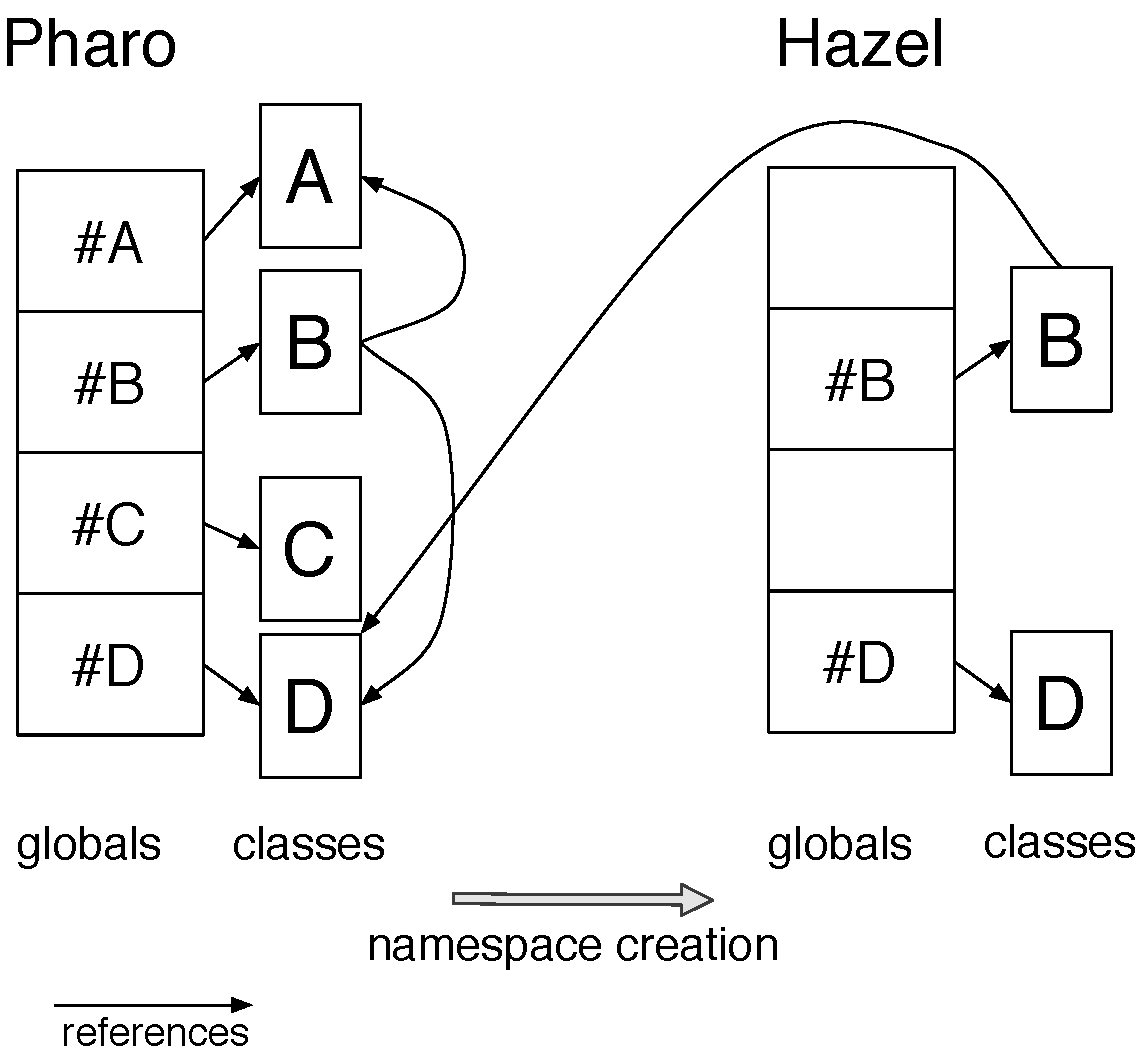
\includegraphics[height = 10cm]{figures/CleaningUnnecessaryRef}
%	\caption{Kernel Isolation}
%	\label{KernelIsolation}
%\end{figure}
%
%
%%% ------------------------------------------------------------ %%
%%
%%	From here I start trying no to use I anymore ^^
%%
%%% ------------------------------------------------------------ %%
%
%Now the Hazel SystemDictionary need to be fixed in order to only have methods depending on itself. To do that, all the methods from all the classes from Hazel SystemDictionary are browsed in order to fix their literals. At this step, we are sure that all the classes needed have already been copied. The problem is that in literals, their also references to global variables, class variables and pool variables, so we just have to check the case which is easy now \gls{TextConstants} (see section~\ref{TextConstants} page~\pageref{TextConstants}) is well restructured.
%
%In fact, those two steps (the copy and the fix) are done in only one pass to gain performance.
%
%Finally, some \glspl{primitive}\footnote{Especially \ct{becomeForward:} and \ct{primitiveChangeClassTo:}} were used to change the structure of the SystemDictionary to have it build with Hazel objects.
%
%Now all references are fixed, so Hazel SystemDictionary is now isolated from the \gls{\gls{Pharo}} world (see Figure~\ref{KernelIsolated}).
%
%\begin{figure}[ht]
%	\centering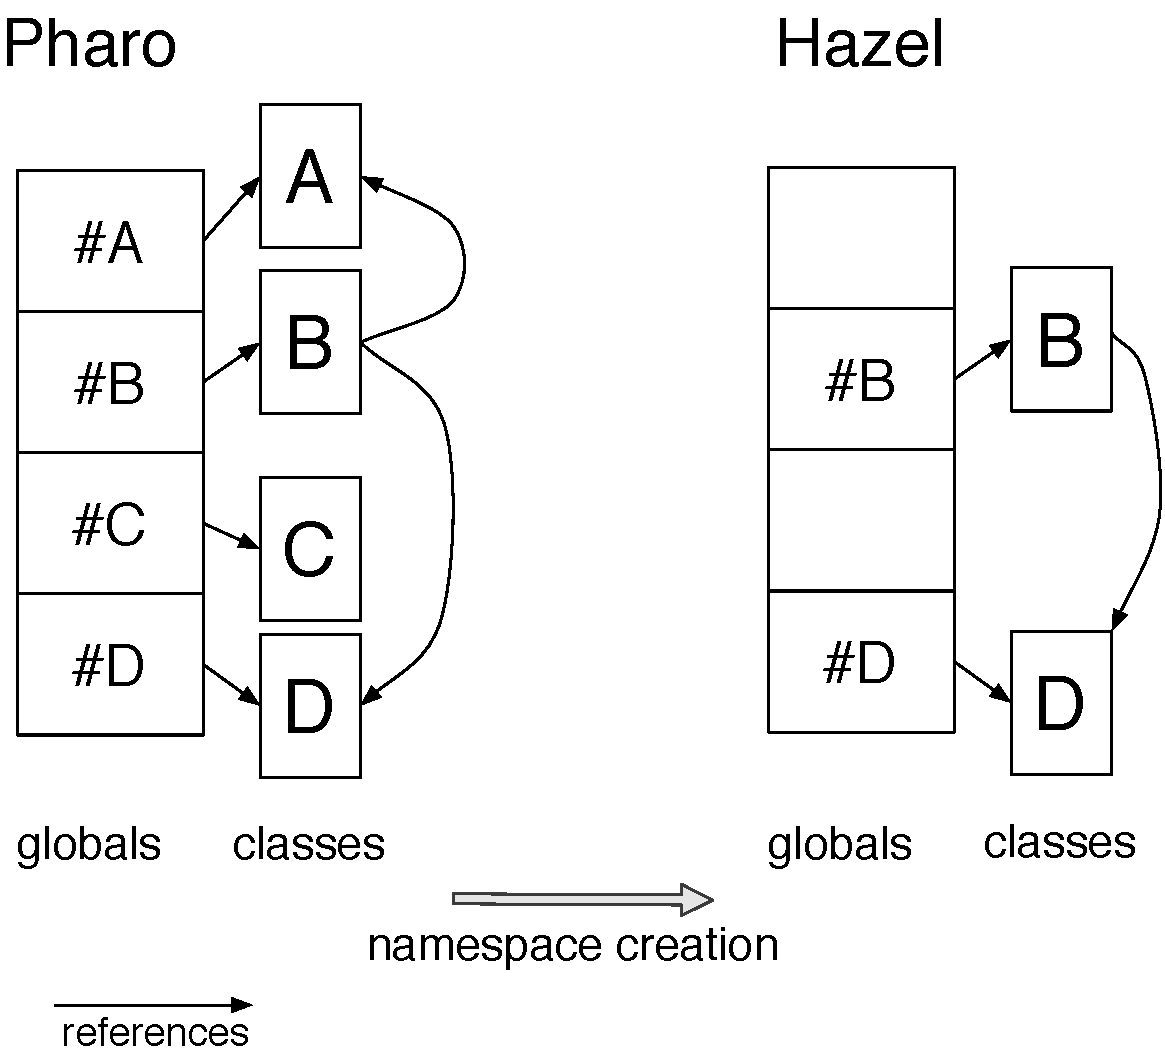
\includegraphics[height = 10cm]{figures/selfContainReference}
%	\caption{Kernel Isolated}
%	\label{KernelIsolated}
%\end{figure}


Now that the kernel is created, we need to isolate it by removing dependencies 
to the \gls{Pharo} world. There is two different types of dependencies which need to be fixed.

\subsection{References to unwanted classes}

\goal Here we want to remove dependencies from Hazel classes to \gls{Pharo} classes we haven't copied.

\problems
\begin{itemize}
	\item How to detect unwanted references ?
	\item How to remove those dependencies ?
	\item How to be sure it will not crash the system ?
\end{itemize}

\solutions
\begin{itemize}
	\item There are two places where unwanted references can be found:
		\begin{itemize}
			\item In a method: in a method literal there are references to invoke classes (see page~\pageref{literal}). Due to that, we can found references to unwanted classes;
			\item In a class variable\footnote{a class variable is a variable shared by all the instances of a class}: we can have an instance of an unwanted class or just an unwanted class itself.
		\end{itemize}
		The solution adopted is to check its \ct{methodDictionary} and class variables during class copy. If unwanted references are found, the following solution is applied.
	\item This is the key point of this cleaning step.
	
	For class variables, the solution was to set them to nil (in the minimal kernel creation process, only one class variable had to be set this way (\ct{HaloFont} from \ct{StandardFonts}).

		
	For methods we have considered several solutions. Our first thought was to remove the method and to recursively remove the sender of the method. But due to class structure, we removed that way almost all methods of the kernel. Then we have though to create a \emph{NullPattern} object implementing all the methods removed. The problem was to find which kind of answer is expected from each method, and how to dynamically replace the sender in the code source. Finally we chose to remove the method and to keep the senders.
	\item We haven't found a solution to this question. %Except if you have control on each methods in your kernel, it will be almost impossible to be sure that your system is safe.
As long as your system can be changed, you can't certify that your kernel is totally functional.
We are working on a better isolation of the \gls{Pharo} kernel to reduce as much as possible the number of references (see Section~\ref{KernelFixes} page~\pageref{KernelFixes} ).
\end{itemize}

\inanutshell We have removed the references to unwanted class (see Figure~\ref{RemoveDependencies}), but because of that the integrity of the kernel may be corrupted.

%%NA: mettre la figure sous SVN
\begin{figure}[ht]
	\centering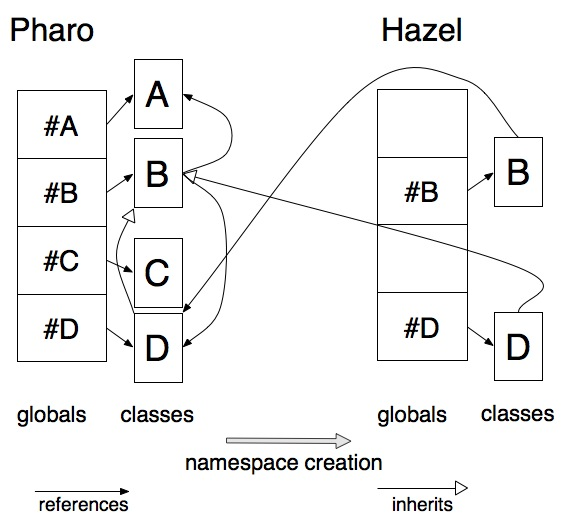
\includegraphics[width = 8cm]{figures/CleaningUnnecessaryRefWithInh}
	\caption{Step 2 - Remove references to unwanted classes}
	\label{RemoveDependencies}
\end{figure}

\newpage
\subsection{Reroute dependencies from original classes to Hazel classes}

\goal Here we want to reroute dependencies from \gls{Pharo} classes to Hazel classes to have only intern references in the Hazel kernel. Those references are stored into methods literals.

\problems
\begin{itemize}
	\item How to change those references ?
	\item How to check what the kernel contains ?
\end{itemize}

\solutions 
\begin{itemize}
	\item This part is quite simple because the field was well prepared. Only methods refering copied classes are not fixed yet. So for those classes, the methodDictionary had just to be parsed in order to fix literals. And for fixing literals, we just change the \gls{Pharo} associations to their corresponding Hazel one (and we are sure it exists).
	\item To check what the new image actually contains, and to be able to modify it f needed, we have modified a bit a couple of tools to be able to browse the living kernel before its serialization.
\end{itemize}

\inanutshell We now have a kernel isolated with only internal references (see Figure~\ref{RerouteDependencies}).

\begin{figure}[ht]
	\centering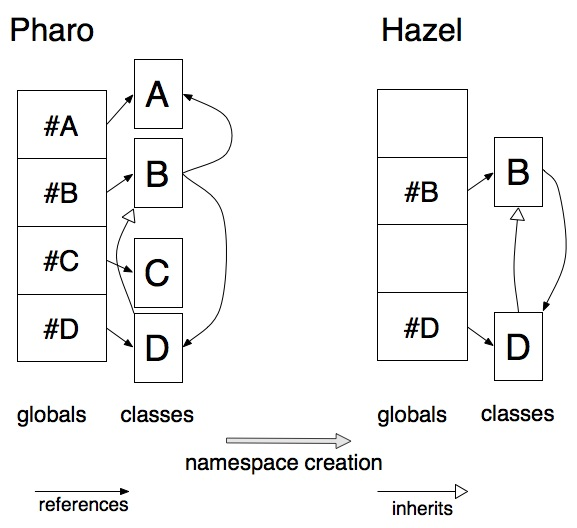
\includegraphics[width = 8cm]{figures/selfContainReferenceWIthInh}
	\caption{Step 3 - Reroute the remaining dependences}
	\label{RerouteDependencies}
\end{figure}









\label{KernelIsolation}
	\section{Image creation}\goal The goal of this part is to successfully build a new image starting from an isolated kernel. An image is a snapshot of living objects binary saved in a file. They basically contains classes and some living instances.
%\sd{Explain Special Objects array}
%done in the Smalltalk presentation part

\problems
\begin{itemize}
	\item Which technique should we use to create the image ?
	\item How to successfully replace the \gls{Special Objects Array} ?
\end{itemize}

\solutions
\begin{figure}[ht]
	\centering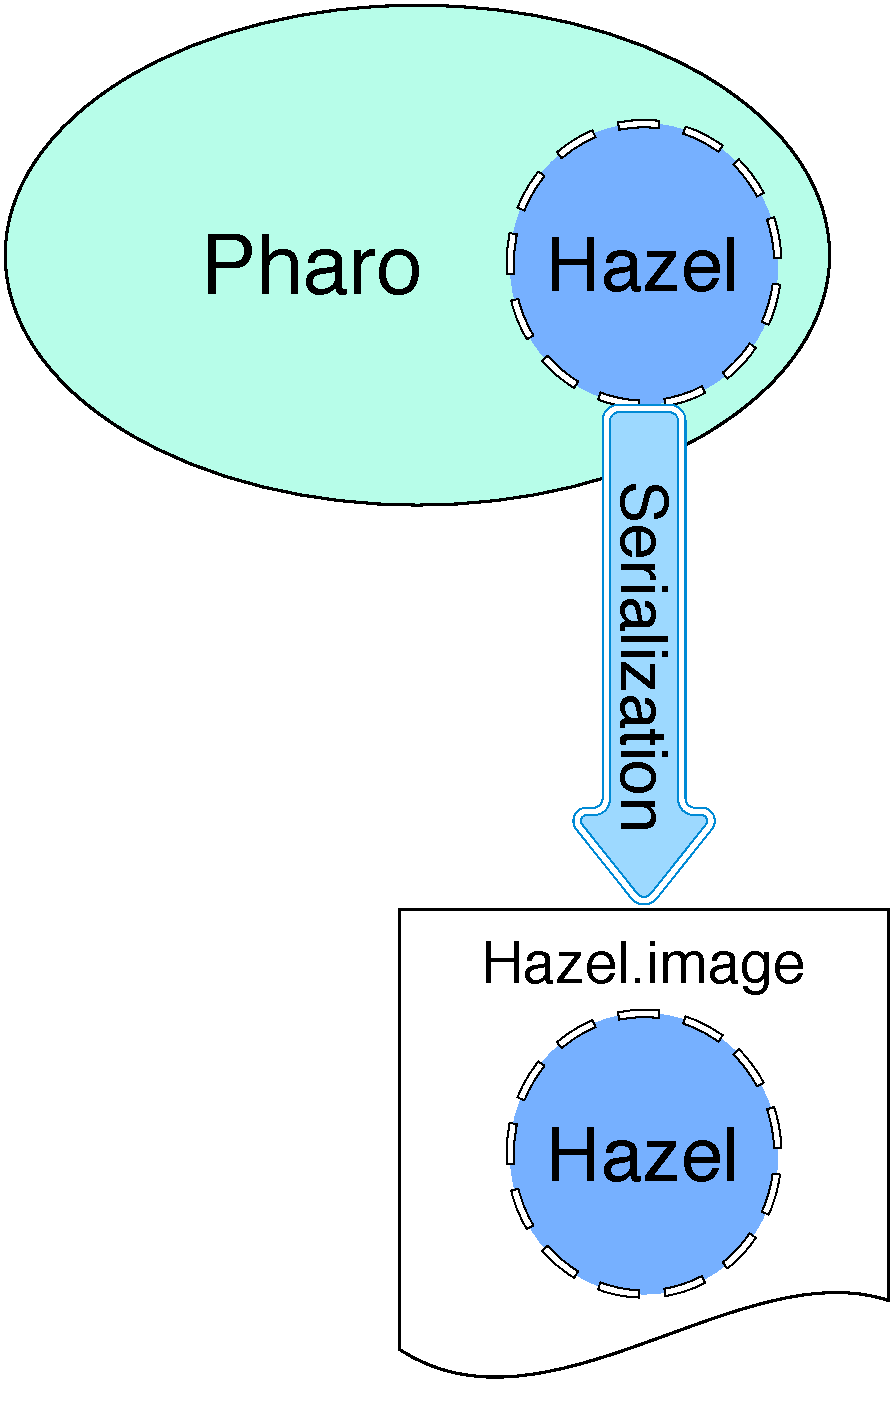
\includegraphics[width = 4.5cm]{figures/MSSolution}
	\caption{Micro Squeak - Serialization of needed objects}
	\label{MSSolution}
\end{figure}
\begin{figure}[ht]
	\centering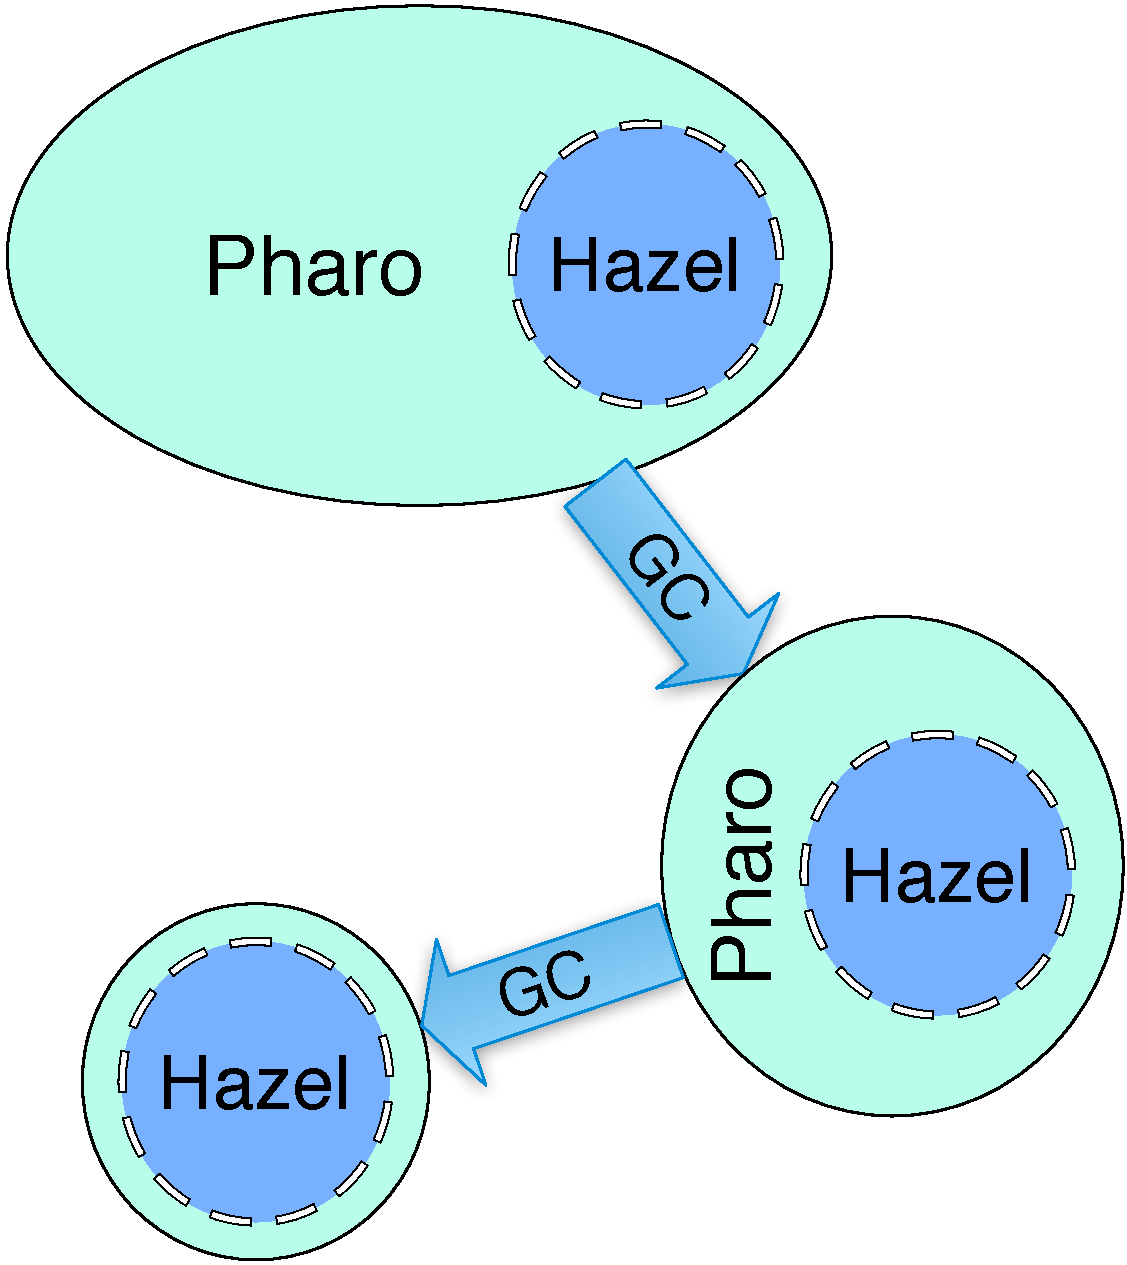
\includegraphics[width = 4.5cm]{figures/HazelSolution}
	\caption{Hazel - Garbage Collection of unneeded objects}
	\label{HazelSolution}
\end{figure}

Two solutions have been tested to create the image:
\begin{itemize}
	\item The first solution was to take a lively image and to dynamically switch the \gls{Special Objects Array} in order to make the unneeded object garbage collected (see \emph{\gls{Garbage Collector}} page~\pageref{glossary}). The difficulty of this method is that we are drastically modifying the image during its own execution. Some objects can easily be changed (i.e. \ct{nil} or \ct{Character}) when some others freeze the Virtual Machine (i.e. \ct{String} or \ct{Semaphore}). We think it's due to the fact that during the execution of the switching method, we are modifying the method context, and the Virtual Machine points to unaccessible pointers and we got an error\footnote{\ct{segmentation fault}} (see Figure~\ref{HazelSolution}).
	\begin{itemize}
		\item To replace the \gls{Special Objects Array}, the idea was to take the current \gls{Special Objects Array}, which is a \ct{Dictionary}, and to replace its values. The problem is that some values called all the time by the image are buffered in the Virtual Machine (those values are \ct{nil},\ct{true} and \ct{false}) and updated at the opening of the image. So we have decided to use the \glspl{primitive} \ct{become:} and \ct{becomeForward:} which basically switch references between the receiver and the argument.
		\item Because some objects can't easily be switched, we have considered another approach.
	\end{itemize}
	\item The second solution, which is also the \gls{Micro Squeak} solution, consists in collecting then serializing all the needed objects into a new image (see Figure~\ref{MSSolution}). But since the tool used for \gls{Micro Squeak} was not maintained anymore and based on a really old version of Pharo, first we had to make it works.
\end{itemize}

\inanutshell We can produce a new image based on the previously created kernel.
	\section{Image initialization}\goal The goal here is to properly initialize the newly created image to make it a real autonomous system.

\problems
\begin{itemize}
	\item What need to be initialized ?
	\item How to reinitialize class variables ?
	\item How to reinitialize classes in the correct order ?
\end{itemize}

\solutions
\begin{itemize}
	\item We know that each class variable has been set to nil during the process, so they need to be initialized to make the system works. But are there any references to a singleton that may have not been initialized ? I still do not know the answer, neither how to find such dependencies, except by checking each dependency by hand.
	\item Class variables should be initialized when the class they belong to is initialized. To ensure that, we checked by hand all classes which belong to the kernel, and ensured that class variables are initialized. If not, we have fixed it.
	\item But then, how to initialize classes ? You can have situations where two classes depend on each other for initialization (see the following example).
	\begin{code}{}\label{initializationCross}
A class>>#initialize
	
\tab myClassVarWhichShouldEqual1 := 1.
\tab myClassVarWhichShouldEqual2 := B myClassVarWhichShouldEqual2.
	
B class>>#initialize
	
\tab myClassVarWhichShouldEqual1 := A myClassVarWhichShouldEqual1.
\tab myClassVarWhichShouldEqual2 := 2.
	\end{code}
In this case, which class to initialize first, A or B ? Since there is no obvious answer and that usually such circular dependencies are pointing to a bad design, the solution is to fix this kind of dependencies.
\end{itemize}
	




%------------------------------------------------------------%
%									%
%		SYSTEM PREPARATION			%
%									%
%------------------------------------------------------------%
\chapter{System Preparation}
To ease the kernel creation process, the system has had to be fixed or at least bugs have had to be flagged. This way we can at least point the structural anomalies and fix them to reduce the number of dependencies. In this optic, we have work on 3 topics:
\begin{itemize}
	\item Text Constants;
	\item Kernel fixes;
	\item Pharo dependencies.
\end{itemize}

	\section{Text Constants}\label{TextConstants}\ct{TextConstants} used to be an old pool dictionary stored as a global variable which was used to store and share information between text related classes. Since the old way of managing pool dictionaries was not good (using global dictionaries), \ct{SharedPool}s have been introduced. A \ct{SharedPool} is a special class designed to store constants variables and to be shared between other classes. You easily use them by specifying the \ct{poolDictionaries} field of a class.

Back in 2006 all dictionaries which only store constants were migrated except TextConstants. The reason of the non migration was probably that it was too deep in the system and that it involved low level fixes.  In addition some applications started to use \ct{TextConstants} not only to share constants but also to act as a bag to store temporary values, defeating the purpose of a Pool Dictionary. 

Due to that, if one browses all classes, and for each browse poolDictionaries, you can have a \ct{SharedPool} (i.e. a \ct{Class}) or \ct{TextConstants} (i.e. a \ct{Dictionary}). Of course those two objects don't have the same interface. So instead of differentiating cases, we have decided to fix the situation and to finally convert \ct{TextConstants} into a \ct{SharedPool}.

\goal
Write a script which can automatically retrieve information from \ct{TextConstants} (as a Dictionary), create a \ct{SharedPool} class named \ct{TextConstants}, then fill up this class with the retrieved information.

\problems
\begin{itemize}
	\item How to differentiate constant values from variable ones ?
	\item Where those methods can store information they used to store in \ct{TextConstants} ?
	\item How avoid to rewrite all the methods ?
\end{itemize}

\solutions
\begin{itemize}
	\item To identify the problems, we read all methods invoking \ct{TextConstants} and finally found a method in \ct{Text class} which initialize \ct{TextConstants}, even if it is in a strange way. So we have invoked this method but on a dummy dictionary instead of \ct{TextConstants} to be able to retrieve all the variables name and value. With those information, it was easy to dynamically defined \ct{TextConstants} and it \ct{initialize} method.
	\item We have decided to add a class variable in \ct{TextConstants} named \emph{TextSharedInformation} which is a \ct{Dictionary} used to store values.
	\item To avoid to rewrite all by hand, we built a script that automatically adds \ct{TextConstants} in the poolDictionaries of classes which need it. When \ct{TextConstants} was used has a \ct{Dictionary}, the code is changed to invoke \emph{TextSharedInformation} instead. But when \ct{TextConstants} is used as a value holder, we had to change methods manually. By chance, only two methods needed to be rewritten this way.
\end{itemize}
	
\inanutshell now \ct{TextConstants} is a SharedPool and the whole system has been changed in order to use the new design of \ct{TextConstants}. All variables founded in the field poolDictionaries are classes.
	

	\section{Kernel fix}\label{KernelFixes}In order to reduce the amount of bad dependencies during the kernel isolation (see section~\ref{KernelIsolation} page~\pageref{KernelIsolation}).

\goal Minimise Pharo kernel dependencies by fixing classes to ease the Hazel kernel isolation.

\problems 
\begin{itemize}
	\item How to identify bad dependencies ?
	\item How to fix them ?
\end{itemize}

\solutions
\begin{itemize}
	\item To identify bad dependencies, we have used \gls{Moose} on \gls{Pharo} 1.2 and have manually flag each dependencies.
	\item To fix them there is no magic formula, we have spent time on it, and we are far from having fix all bad dependencies. But a bug entry was opened on the developers platform for each bad dependence.
\end{itemize}

\inanutshell 20 dependencies have already been fixed, but 40 bug entries are still open waiting for a fix.
	\section{Pharo dependencies}Here the topic is the same that the previous one. We want to flag dependencies in order to isolate modules, but here it's for the whole system.

\goal Analyze (and fix) all \gls{Pharo} bad dependencies in order to have isolated modules easily pluggable and un-pluggable and not circular references in class initialization.

\problems 
\begin{itemize}
	\item Which tool to use to analyze a whole system ?
	\item How to automatize the creation of a new bug entry ?
	\item How to break circular references ?
\end{itemize}

\solutions 
\begin{itemize}
	\item Moose have been used here too to build a tool that flag Pharo packages dependencies (about 1300 dependencies);
	\item We haven't found how to use the Google interface to automatize the creation of bug entries, so we have to add each bad dependence one by hand.
	\item To break circular references, there is no automatic answer. Each case has to be analyzed and deeply understood before being fixed.
\end{itemize}

\inanutshell Now that all the bad dependencies are flagged, it's easier to focus on important things to fix.




\chapter{Conclusion}
	\section{Technical results}I have technically learned a lot during my internship at many levels. Here is a non-exhaustive list of things I have learned or deepened.

\paragraph{Smalltalk.} I already knew \gls{Smalltalk} before the beginning of the internship. But I have improved my knowledge about the \gls{Smalltalk} language especially because I used to borrow a lot of books from the lab, in particular the ones about dynamic languages. Thanks to \gls{Smalltalk}, and the fact that you can browse living objects, I understand how an object-oriented language works more deeply.

\paragraph{Pharo.} By analyzing the \gls{Pharo} kernel then the whole system, I have read a lot of code and this way learned a lot about the \gls{Pharo} internal structure. It allows me to think at the precise definition of a kernel, which classes are needed to run a system. Thanks to these analyses, I now have a better comprehension of modular packages.

\paragraph{The Virtual Machine.} I have learned bases of how the \gls{VM} works and how to create a new version of the current \gls{VM} using \ct{VMMaker}. I have also learned how to add new primitives in the system. I really would like to know more about the \gls{VM}, because it used to looks like a black box even if the system can't work without the \gls{VM}.

\paragraph{English.} The team being multi-cultural with people from several countries, the english is used all the time for the internal communications. Moreover, all the mails shared in the Pharo mailing list are in english too. I started to learn how to write a research paper in english.

\paragraph{SVN.} The team is using \gls{SVN} for storing internal information, so I had to learn how it works.
	\section{Human results} \subsection{Integrate a research team}

Even while I  learned a lot technically, humanly I  discovered a new working environment inside the RMoD team, where communication and autonomy are really important.
\begin{itemize}
	\item The communication is the backbone of the research work whether written or oral Another member of the team was working on a similar project (\emph{PineKernel}) and each day we sent an email to the whole team with a sum up of our daily work. This way we were aware of each other work, and we shared a lot of knowledge. Moreover, I have often take a seat and ask a question to another team member, and spent hours sharing ideas and quickly test them. A large part of ideas used in Hazel were born this way, and it was really pleasant to work this way. 
	\item The autonomy in work was import too because I had to make my own schedule and to learn how to manage my time. Moreover, I was alone working on the Hazel project, so I had to set a rhythm by myself. In the other hand, I forced myself not to work at home, to keep a regular rhythm which is big change compared to the \gls{IUT}.
\end{itemize}

I also had multiple points of view on the work of a researcher, which is the job I would like to do. Moreover, the team being multi-cultural, I've learned some cultural parts from Argentinian culture (like Alfajoles), or Ukrainian one. It was really cool to practice my english with people from all over the world.

\subsection{Pharo, a living community}

Beside working for the \gls{INRIA}, I worked as a member of the active \gls{Pharo} community. I had developed some projects before being a member of the team. Those projects have been improved and integrate into the current version of \gls{Pharo}. These improvements have been done with the help of other members of the community especially during Sprints (coding session). This community is really reactive and any question, from the dumbest one to the more specific one, can be asked on the mailing list you will always have an answer.


\inanutshell It was really a good experience that I hope I could reproduce. I really like to manage a project by myself, and to schedule my work alone. Moreover I really like to work on a research theme.
	\section{Conclusion} \paragraph{Context:} After the John Maloney's MicroSqueak, project has been released, we had a proof that the creation of a new kernel was possible, and we wanted to have this concept in \gls{Pharo}. Some other projects\footnote{mainly Chacharas, Spoon } have provided the tools to create new kernel, but with a different approach and not working anymore. Seed is the first project inpsired by \gls{Micro Squeak}.

\goal The goal of the project was to implement a process able to dynamically create a new kernel starting from a living image and a collection of classes the new kernel must provide. In parallel, I had to fix the \gls{Pharo} structure in order to ease the previous process. 

\problems The most important problems encountered were:
	\begin{itemize}
		\item What is \gls{Pharo} kernel ?
		\item How to collect needed classes ?
		\item How to create another kernel in a living image ?
		\item How to isolate the kernel ?
		\item Does the \gls{Pharo} structure allow you to easily separate modules ?
		\item How to bootstrap the kernel ?
		\item How to create a new image with this kernel ?
	\end{itemize}

\paragraph{Solution:} After structural analysis, I have implemented a script which takes a list of classes as an argument, and build an autonomous kernel with all the classes needed and wanted. I have also provided another script to serialize this kernel as a new image which is a real system fully working.
\paragraph{Next Steps:}
The next steps will be to explore another way for filling the new name space. Instead of copying objects for the current system, trying to have a file based declarative boostrap. We could also fix the whole structure to ease the kernel isolation, and this way having a better isolated kernel in \gls{Pharo}.

\paragraph{Conclusion:} As a conclusion, Hazel provides tools to create a new isolated kernel, and also a new image with this kernel fully working. Working on the definition of a kernel, especially in \gls{Pharo} allowed us to define which classes \emph{are composing} the current kernel and which one \emph{should compose} the kernel. 

Working on the system structure had also revealed some problems in the packages architecture and dependencies. 

%\backmatter
\newpage

\printglossaries\label{glossary}

%Do not care anymore


\bibliographystyle{abbrv}
\bibliography{rmod,others}


\pagestyle{empty}
\newpage

\ifthenelse{\isodd{\value{page}}}
{}%impaire
{\hbox{}\clearpage}%paire

\addcontentsline{toc}{section}{Abstract}
\vfill 

\resume*{R\'{e}sum\'{e}}

Dans le cadre de mon stage de fin d'\'{e}tudes, j'ai eu en charge le projet \textbf{Hazelnut} au sein de l'\'{e}quipe RMoD au sein de l'INRIA (Institut National de Recherche en Informatique et en Automatique) de Lille. Le projet Hazelnut consiste en la cr\'{e}ation dynamique d'un nouveau noyau d'ex\'{e}cution \`{a} partir d'une \mbox{impl\'{e}mentation} de Smalltalk, Pharo. 

Ce projet doit permettre de concevoir aisement des noyaux minimaux pouvant servir \`{a} des syst\`{e}mes embarqu\'{e}s aussi bien qu'\`{a} red\'{e}finir facilement la fa\c{c}on dont le noyau (et donc le syst\`{e}me) fonctionne.


\vfill

\resume*{Abstract}

During my internship at INRIA (Institut National de Recherche en Informatique et en Automatique) in the RMoD team, I had in charge the \textbf{Hazelnut} project which consists in the dynamic creation of a new kernel from Pharo, an implementation of Smalltalk.

This project will be used to create minimal kernel for embedded systems or to easily redefine the way the kernel (and the whole system) works.

\vfill

\newpage
\end{document}

%%% Local Variables: 
%%% coding: utf-8
%%% mode: latex
%%% TeX-master: "main"
%%% TeX-PDF-mode: t
%%% End:

\end{document}